% =====================================================================
%  GrabGuard — GrabHack 2026 Grand Finale Pitch Deck
%  Problem Statement 3 — Personalized GenAI Financial Services
%  Compile:  pdflatex grabguard_pitch.tex   (twice for footer counters)
% =====================================================================
\documentclass[aspectratio=169,xcolor={dvipsnames,table}]{beamer}

% ---------------------------------------------------------------------
%  Packages
% ---------------------------------------------------------------------
\usepackage[utf8]{inputenc}
\usepackage[T1]{fontenc}
\usepackage{lmodern}
\usepackage{microtype}
\usepackage{xcolor}
\usepackage{colortbl}
\usepackage{booktabs}
\usepackage{array}
\usepackage{multirow}
\usepackage{adjustbox}
\usepackage{graphicx}
\usepackage{fontawesome5}
\usepackage{tikz}
\usetikzlibrary{
  arrows.meta,
  positioning,
  shapes.geometric,
  shapes.misc,
  fit,
  calc,
  backgrounds,
  decorations.pathreplacing,
  shadows,
  shadows.blur
}

% ---------------------------------------------------------------------
%  Brand palette
% ---------------------------------------------------------------------
% Neutral dark background, WHITE-dominant text, green ONLY as brand accent.
\definecolor{GrabGreen}{HTML}{00B14F}    % brand green — accents, key numbers, icons
\definecolor{GrabAccent}{HTML}{00E676}   % bright green — sparingly, for top highlights
\definecolor{GrabDark}{HTML}{0E1116}     % neutral dark slide background
\definecolor{GrabMid}{HTML}{1A1F25}      % neutral dark card background (no green tint)
\definecolor{GrabGray}{HTML}{A6AEB5}     % neutral mid-gray for secondary text
\definecolor{GrabRed}{HTML}{FF5C5C}
\definecolor{GrabWhite}{HTML}{FFFFFF}    % pure white body text

% ---------------------------------------------------------------------
%  Beamer theme
% ---------------------------------------------------------------------
\setbeamercolor{background canvas}{bg=GrabDark}
\setbeamercolor{normal text}{fg=GrabWhite}
\setbeamercolor{frametitle}{fg=GrabWhite,bg=GrabDark}
\setbeamercolor{title}{fg=GrabWhite}
\setbeamercolor{itemize item}{fg=GrabGreen}
\setbeamercolor{itemize subitem}{fg=GrabGray}
\setbeamercolor{enumerate item}{fg=GrabGreen}
\setbeamercolor{block title}{fg=GrabWhite,bg=GrabMid}
\setbeamercolor{block body}{fg=GrabWhite,bg=GrabMid}
\setbeamercolor{alerted text}{fg=GrabGreen}
\setbeamerfont{frametitle}{series=\bfseries,size=\Large}
\setbeamerfont{title}{series=\bfseries,size=\huge}

\setbeamertemplate{navigation symbols}{}
\setbeamertemplate{itemize item}{\color{GrabGreen}\scriptsize\faSquare}
\setbeamertemplate{itemize subitem}{\color{GrabGray}\scriptsize\faMinus}

% Frame title with 3pt left GrabGreen accent rule
\setbeamertemplate{frametitle}{%
  \nointerlineskip%
  \vspace*{0.45em}%
  \hspace*{1em}%
  
\begin{tikzpicture}[baseline=(x.base)]
    \fill[GrabGreen] (-4pt,-1.2ex) rectangle (-1pt,2.4ex);
    \node[anchor=west,text=GrabWhite,font=\large\bfseries,inner sep=0pt]
      (x) at (4pt,0.7ex) {\insertframetitle};
  \end{tikzpicture}%
  \vspace*{0.2em}%
}

% Footer
\setbeamertemplate{footline}{%
  \leavevmode
  \hbox{%
    \begin{beamercolorbox}[wd=.65\paperwidth,ht=3ex,dp=1ex,left]{}
      \hspace*{1em}{\scriptsize\color{GrabGray} GrabHack 2026 \textemdash{} Problem Statement 3}%
    \end{beamercolorbox}%
    \begin{beamercolorbox}[wd=.35\paperwidth,ht=3ex,dp=1ex,right]{}
      {\scriptsize\color{GrabGray}\insertframenumber\,/\,\inserttotalframenumber}\hspace*{1em}%
    \end{beamercolorbox}%
  }%
}

% ---------------------------------------------------------------------
%  Custom commands
% ---------------------------------------------------------------------
\newcommand{\tagpill}[1]{%
  \tikz[baseline=(p.base)]{%
    \node[fill=GrabGreen!20,text=GrabAccent,rounded corners=4pt,%
          inner xsep=7pt,inner ysep=3pt,font=\scriptsize\bfseries] (p) {#1};%
  }%
}

% Note: metric label is laid out with align=center + text width, so the
% caller MUST NOT use \\ in the label argument (the outer tabular would
% intercept it as a row break before our inner node ever sees it). Long
% labels wrap automatically thanks to text width.
\newcommand{\metricbox}[2]{%
  \begin{tikzpicture}
    \node[fill=GrabMid,rounded corners=6pt,%
          minimum width=3.0cm,minimum height=1.9cm,%
          text width=2.7cm,
          inner sep=4pt,align=center,
          drop shadow={shadow xshift=0pt,shadow yshift=-1pt,opacity=0.35}] {%
      \centering
      {\color{GrabAccent}\bfseries\Large #1}\par
      \vspace{2pt}
      {\color{GrabGray}\scriptsize #2}%
    };
  \end{tikzpicture}%
}

% Dashed-bordered TikZ placeholder for missing screenshots
\newcommand{\placeholder}[1]{%
  \par\noindent
  \begin{tikzpicture}
    \node[draw=GrabGray,dashed,thick,rounded corners=6pt,%
          minimum height=3.6cm,
          text width={\dimexpr\linewidth-1.4cm\relax},
          text=GrabGray,align=center,font=\itshape\footnotesize,
          fill=GrabMid,inner sep=12pt] {%
      \faImage\quad #1\\[6pt]
      {\scriptsize(drop a PNG at this filename to replace this placeholder)}%
    };
  \end{tikzpicture}%
}

% Screenshot include with GrabGreen border + caption + IfFileExists guard
\newcommand{\screenshot}[2]{%
  \IfFileExists{#1}{%
    \begin{tikzpicture}
      \node[draw=GrabGreen,line width=0.8pt,rounded corners=4pt,inner sep=2pt]
        {\includegraphics[width={\dimexpr\linewidth-10pt\relax}]{#1}};
    \end{tikzpicture}%
  }{%
    \placeholder{#2}%
  }\\[3pt]
  {\scriptsize\color{GrabGray}\textit{#2}}%
}

% Coloured agent-tag for the live-stream mock console
\newcommand{\agtag}[1]{\textcolor{GrabAccent}{\ttfamily [#1]}}

% =====================================================================
\begin{document}

% ─── SLIDE 1 — TITLE ───
\begin{frame}[plain]
  \begin{tikzpicture}[remember picture,overlay]
    % slim GrabGreen top accent band (no longer full-bleed)
    \fill[GrabGreen]
      (current page.north west) --
      (current page.north east) --
      ([yshift=-0.6cm]current page.north east) --
      ([yshift=-0.9cm]current page.north west) -- cycle;
    \node[anchor=north east,text=GrabDark,font=\bfseries\scriptsize]
      at ([xshift=-1.0cm,yshift=-0.18cm]current page.north east)
      {GrabHack 2026 \textemdash{} Grand Finale};
    \node[anchor=north west,text=GrabDark,font=\bfseries\scriptsize]
      at ([xshift=1.0cm,yshift=-0.18cm]current page.north west)
      {\faShield\quad Problem Statement 3};
  \end{tikzpicture}

  \vspace*{2.4cm}
  \begin{center}
    {\fontsize{38}{42}\selectfont\bfseries\color{GrabWhite} GrabGuard}\\[0.35cm]
    {\large\color{GrabWhite} AI-Powered Fraud Mitigation for the Gig Economy}\\[0.2cm]
    {\footnotesize\color{GrabGray} Personalized GenAI Financial Services \textemdash{}
     a gig-worker-aware fraud \& wellness agent for the GXS / Grab partner stack}\\[0.7cm]
    \tagpill{\faBolt\, Groq LLaMA\,3.3 70B}\quad
    \tagpill{\faNetworkWired\, Multi-Agent AI}\quad
    \tagpill{\faChartPie\, Explainable ML}\quad
    \tagpill{\faUserShield\, Financial Digital Twin}\\[0.7cm]
    {\scriptsize\color{GrabGray}
      \faGithub\enspace github.com/ansh-0069/fraud\_agent
      \quad\textbar\quad
      \faCalendar\enspace May 2026}
  \end{center}
\end{frame}

% ─── SLIDE 2 — THE PROBLEM ───
\begin{frame}[t]{The Problem}
  \begin{columns}[T,onlytextwidth]
    \begin{column}{0.54\textwidth}
      {\color{GrabWhite}\bfseries\large Why generic fraud systems break for gig workers}\\[0.4em]
      {\color{GrabGray}\scriptsize Legacy banking models assume salaried, regular cash flow.
      Gig income is volatile by design \textemdash{} and the model punishes the worker for it.}
      \vspace{0.3em}

      \begin{itemize}\footnotesize\setlength\itemsep{0.2em}
        \item \textcolor{GrabRed}{\faExclamationTriangle}\,
              \textbf{Surge Friday looks like fraud.} \$2{,}100 surge income is an outlier to fixed-threshold models.
        \item \textcolor{GrabRed}{\faExclamationTriangle}\,
              \textbf{72-hour freezes} on week-to-week workers $=$ missed rent, missed shifts.
        \item \textcolor{GrabRed}{\faExclamationTriangle}\,
              \textbf{Black-box decisions} fail MAS FEAT (Fairness, Ethics, Accountability, Transparency).
        \item \textcolor{GrabRed}{\faExclamationTriangle}\,
              \textbf{No cross-session memory.} Every appeal starts from zero \textemdash{} no trust accrued.
      \end{itemize}
    \end{column}

    \begin{column}{0.43\textwidth}
      {\color{GrabGreen}\bfseries\small SCALE OF THE PROBLEM}\\[0.25em]
      \renewcommand{\arraystretch}{1.15}
      \arrayrulecolor{GrabGreen}
      \scriptsize
      \begin{tabular}{>{\color{GrabGray}}l >{\raggedleft\arraybackslash\color{GrabWhite}\bfseries}p{2.2cm}}
        \toprule
        Gig workers in SEA & 9M+ \\
        Annual fraud losses & \$3.6B \\
        Industry FPR on gig profiles & 21\% \\
        Avg freeze on flagged accounts & 72h \\
        Income lost per freeze & \$300\textendash 500 \\
        Drivers who quit post-freeze & 38\% \\
        \bottomrule
      \end{tabular}
      \arrayrulecolor{black}
      \normalsize
      \vspace{0.4em}

      
\begin{tikzpicture}
        \node[fill=GrabMid,rounded corners=6pt,text width=0.92\linewidth,
              inner sep=6pt,text=GrabWhite,font=\scriptsize] {
          \textcolor{GrabGreen}{\bfseries Bottom line: }
          banks lose trust, drivers lose income, regulators lose patience.
        };
      \end{tikzpicture}
    \end{column}
  \end{columns}
\end{frame}

% ─── SLIDE 3 — MARKET CONTEXT / WHY NOW ───
\begin{frame}[t]{Market Context \textemdash{} Why Now}
  \vspace*{-0.6em}
  \begin{center}
  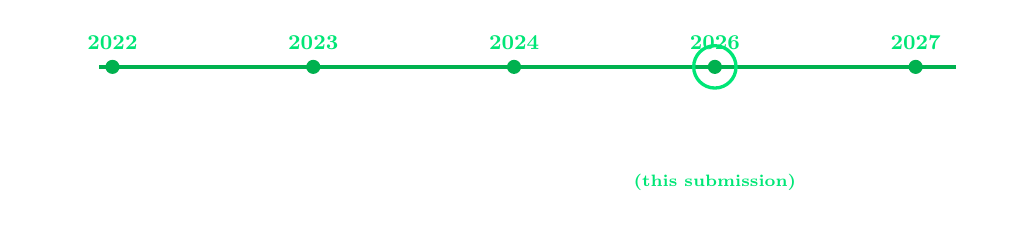
\begin{tikzpicture}[
    yshift=0,
    every node/.style={font=\scriptsize},
    scale=0.85, transform shape
  ]
    % timeline rule
    \draw[GrabGreen,line width=1.4pt] (-0.2,0) -- (12.6,0);
    % milestone nodes
    \foreach \x/\year/\evt in {
      0/2022/{GXS Bank launches},
      3/2023/{FlexiLoan rolls out},
      6/2024/{GXS loan book\\doubles to 200K},
      9/\textbf{2026}/{\bfseries GrabGuard ships},
      12/2027/{GXS profit target}
    }{
      \fill[GrabGreen] (\x,0) circle (3pt);
      \node[above=4pt,text=GrabAccent,font=\small\bfseries] at (\x,0) {\year};
      \node[below=6pt,text=GrabWhite,align=center,text width=2.3cm]
        at (\x,0) {\evt};
    }
    % highlight 2026
    \draw[GrabAccent,line width=1.2pt] (9,0) circle (9pt);
    \node[below=42pt,text=GrabAccent,align=center,text width=2.4cm,font=\scriptsize\bfseries] at (9,0) {(this submission)};
  \end{tikzpicture}
  \end{center}

  \vspace{0.5em}
  \begin{columns}[T,onlytextwidth]
    \begin{column}{0.32\textwidth}
      \begin{tikzpicture}
        \node[fill=GrabMid,rounded corners=6pt,text width=\linewidth-12pt,
              inner sep=6pt] {%
          \textcolor{GrabGreen}{\bfseries\small\faChartLine\, GXS Gap}\\[2pt]
          \textcolor{GrabWhite}{\scriptsize GXS doubled to 200K loans in 6mo on legacy fraud rules tuned for salaried customers. Gig defaults rising.}
        };
      \end{tikzpicture}
    \end{column}
    \begin{column}{0.32\textwidth}
      
\begin{tikzpicture}
        \node[fill=GrabMid,rounded corners=6pt,text width=\linewidth-12pt,
              inner sep=6pt] {%
          \textcolor{GrabGreen}{\bfseries\small\faGavel\, Regulatory Push}\\[2pt]
          \textcolor{GrabWhite}{\scriptsize MAS FEAT demands explainability for every automated financial decision in Singapore by 2026.}
        };
      \end{tikzpicture}
    \end{column}
    \begin{column}{0.32\textwidth}
      \begin{tikzpicture}
        \node[fill=GrabMid,rounded corners=6pt,text width=\linewidth-12pt,
              inner sep=6pt] {%
          \textcolor{GrabGreen}{\bfseries\small\faSearch\, Competitor Gap}\\[2pt]
          \textcolor{GrabWhite}{\scriptsize Revolut, Wise, Aspire treat gig income as risk. None ship gig-native ML + multi-agent + audit in one.}
        };
      \end{tikzpicture}
    \end{column}
  \end{columns}
\end{frame}

% ─── SLIDE 4 — SOLUTION OVERVIEW ───
\begin{frame}[t]{Solution Overview}
  \begin{columns}[T,onlytextwidth]
    \begin{column}{0.56\textwidth}
      {\color{GrabWhite}\bfseries\large Three layers, one promise: gig income is protected, not punished.}\\[0.4em]

      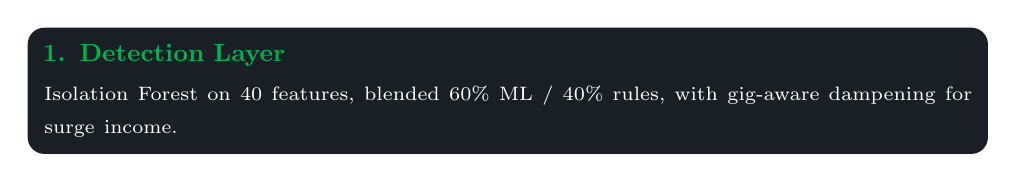
\begin{tikzpicture}
        \node[fill=GrabMid,rounded corners=6pt,text width=\linewidth-10pt,
              inner sep=6pt] {%
          \textcolor{GrabGreen}{\bfseries\small 1. Detection Layer}\\[2pt]
          \textcolor{GrabWhite}{\scriptsize Isolation Forest on 40 features, blended 60\% ML / 40\% rules, with gig-aware dampening for surge income.}
        };
      \end{tikzpicture}\\[4pt]
      
\begin{tikzpicture}
        \node[fill=GrabMid,rounded corners=6pt,text width=\linewidth-10pt,
              inner sep=6pt] {%
          \textcolor{GrabGreen}{\bfseries\small 2. Agent Reasoning Layer}\\[2pt]
          \textcolor{GrabWhite}{\scriptsize 6 specialised agents on Groq LLaMA\,3.3 70B with SSE live-streamed reasoning.}
        };
      \end{tikzpicture}\\[4pt]
      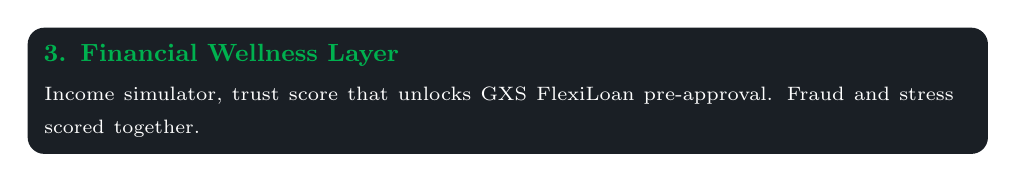
\begin{tikzpicture}
        \node[fill=GrabMid,rounded corners=6pt,text width=\linewidth-10pt,
              inner sep=6pt] {%
          \textcolor{GrabGreen}{\bfseries\small 3. Financial Wellness Layer}\\[2pt]
          \textcolor{GrabWhite}{\scriptsize Income simulator, trust score that unlocks GXS FlexiLoan pre-approval. Fraud and stress scored together.}
        };
      \end{tikzpicture}
    \end{column}

    \begin{column}{0.42\textwidth}
      {\color{GrabGreen}\bfseries\small HEADLINE METRICS}\\[0.25em]
      \begin{tabular}{cc}
        \metricbox{89\%}{False-positive rate reduction} &
        \metricbox{$<$200ms}{Groq agent response time} \\[6pt]
        \metricbox{94.2\%}{Detection precision} &
        \metricbox{9M+}{Gig workers (SEA)}
      \end{tabular}
    \end{column}
  \end{columns}
\end{frame}

% ─── SLIDE 5 — SYSTEM ARCHITECTURE ───
\begin{frame}[t]{System Architecture}
  \begin{center}
  \begin{tikzpicture}[
    every node/.style={font=\scriptsize,align=center},
    agent/.style={rectangle,rounded corners=4pt,fill=GrabMid,draw=GrabGreen,
                  text=GrabWhite,minimum width=1.9cm,minimum height=0.7cm,inner sep=3pt},
    hub/.style={rectangle,rounded corners=4pt,fill=GrabGreen,draw=GrabAccent,
                text=GrabDark,minimum width=2.2cm,minimum height=0.8cm,
                inner sep=3pt,font=\scriptsize\bfseries},
    tool/.style={rectangle,rounded corners=4pt,fill=GrabGreen!18,draw=GrabAccent,
                 text=GrabAccent,minimum width=2.5cm,minimum height=0.7cm,
                 inner sep=3pt,font=\scriptsize\bfseries},
    flow/.style={-{Stealth[length=4.5pt]},draw=GrabGreen,line width=0.7pt},
    sse/.style={-{Stealth[length=4.5pt]},draw=GrabAccent,dashed,line width=0.7pt}
  ]
    % Top row — client → backend → orchestrator
    \node[agent] (react) at (0,3.2) {React + Vite\\Frontend};
    \node[agent] (api) at (3,3.2) {FastAPI\\Gateway};
    \node[hub]   (orch) at (6.5,3.2) {Orchestrator\\Agent};

    \draw[flow] (react) -- (api);
    \draw[flow] (api) -- (orch);

    % Middle row — 6 specialised agents
    \node[agent] (det)   at (-0.2,1.5) {Detection};
    \node[agent] (exp)   at (2.2,1.5)  {Explanation};
    \node[agent] (mem)   at (4.6,1.5)  {Memory};
    \node[agent] (appl)  at (7.0,1.5)  {Appeal};
    \node[agent] (well)  at (9.4,1.5)  {Wellness};
    \node[agent] (audit) at (11.8,1.5) {Audit};

    \foreach \n in {det,exp,mem,appl,well,audit}
      \draw[flow] (orch) -- (\n);

    % Bottom row — tools
    \node[tool] (groq) at (1.0,-0.2) {Groq LLaMA\,3.3 70B};
    \node[tool] (ml)   at (5.5,-0.2) {Isolation Forest + SHAP};
    \node[tool] (db)   at (10.0,-0.2) {SQLite (persistent memory)};

    \draw[flow] (det) -- (ml);
    \draw[flow] (exp) -- (groq);
    \draw[flow] (exp) -- (ml);
    \draw[flow] (mem) -- (db);
    \draw[flow] (appl) -- (db);
    \draw[flow] (well) -- (groq);
    \draw[flow] (audit) -- (db);

    % SSE loopback
    \draw[sse] (orch.north) to[bend left=55]
      node[above,font=\tiny,text=GrabAccent] {SSE stream \textbullet\ real-time reasoning} (react.north);

    % Legend
    \node[anchor=west,text=GrabGray,font=\tiny] at (0,-1.4)
      {\textcolor{GrabGreen}{\faSquare}\ Specialised agent\quad
       \textcolor{GrabAccent}{\faSquare}\ Tool / model\quad
       \textcolor{GrabAccent}{- - -}\ SSE log stream};
  \end{tikzpicture}
  \end{center}
\end{frame}

% ─── SLIDE 6 — INNOVATION 1: GIG-WORKER DAMPENING ───
\begin{frame}[t]{Innovation 1 \textemdash{} Gig-Worker Income Dampening}
  \begin{columns}[T,onlytextwidth]
    \begin{column}{0.54\textwidth}
      {\color{GrabGreen}\bfseries\small THE CORE INSIGHT}\\[0.2em]
      {\color{GrabWhite}\scriptsize A verified gig worker earning surge income is \emph{not} an anomaly to be punished. We encode that into the score.}
      \vspace{0.3em}

      \begin{itemize}\scriptsize\setlength\itemsep{0.15em}
        \item Isolation Forest on 40 features \textemdash{} unchanged.
        \item Verified gig profile: subtract \textbf{0.15} dampening factor.
        \item 30-day rolling income variance window stabilises baseline.
        \item Final = \textbf{0.6$\times$ML} + \textbf{0.4$\times$rule} \textemdash{} prevents gaming.
      \end{itemize}

      \vspace{0.3em}
      {\color{GrabGreen}\bfseries\small BEFORE / AFTER \textemdash{} surge Friday driver}\\[0.15em]
      \scriptsize
      \begin{tabular}{l l}
        \textcolor{GrabRed}{\faTimesCircle}\, \textbf{Without} &
          \$2{,}100 surge flagged, frozen 72h, \$400 lost \\
        \textcolor{GrabAccent}{\faCheckCircle}\, \textbf{With} &
          Dampening applied, \textbf{0.71\,$\to$\,0.56}, approved
      \end{tabular}
      \normalsize
      \vspace{0.3em}

      \tagpill{FPR 21\% $\to$ 2.3\%}\quad
      \tagpill{89\% reduction}
    \end{column}

    \begin{column}{0.44\textwidth}
      \screenshot{screenshots/transaction_monitor.png}{Live transaction feed \textemdash{} surge driver auto-approved with dampening applied}
    \end{column}
  \end{columns}
\end{frame}

% ─── SLIDE 7 — INNOVATION 2: MULTI-AGENT PIPELINE ───
\begin{frame}[t]{Innovation 2 \textemdash{} Multi-Agent Pipeline}
  {\color{GrabGray}\scriptsize Six specialised agents \textemdash{} each with a distinct role and toolset. Orchestrator dispatches; the rest reason.}
  \vspace{0.2em}

  \renewcommand{\arraystretch}{1.1}
  \arrayrulecolor{GrabGreen}
  \scriptsize
  \begin{tabular}{
    >{\color{GrabWhite}\bfseries}l
    >{\color{GrabWhite}}p{4.8cm}
    >{\color{GrabWhite}}p{6.6cm}
  }
    \toprule
    \rowcolor{GrabMid}
    \textcolor{GrabGreen}{Agent} &
    \textcolor{GrabGreen}{Role} &
    \textcolor{GrabGreen}{Key Output} \\
    \midrule
    Orchestrator   & Routes queries, dispatches sub-agents
                   & Final decision + reasoning trace ID \\
    Detection      & Isolation Forest + rules + gig dampening
                   & Risk score, band (APPROVE / REVIEW / FREEZE) \\
    Explanation    & SHAP TreeExplainer + LLaMA narrative
                   & Top-3 features + 2-sentence rationale \\
    Memory         & SQLite trust-score history + pattern recall
                   & Trust score 0\textendash 1, pattern flags \\
    Appeal         & False-positive dispute resolution
                   & Overturn / uphold + SHAP-backed justification \\
    Fin.~Wellness  & Income simulator + runway estimator
                   & Wellness score, runway days, GXS signal \\
    \bottomrule
  \end{tabular}
  \arrayrulecolor{black}
  \normalsize

  \vspace{0.4em}
  \tagpill{\faBolt\, sub-200ms Groq inference}\quad
  \tagpill{\faStream\, SSE streaming}\quad
  \tagpill{\faDatabase\, SQLite persistence}
\end{frame}

% ─── SLIDE 8 — INNOVATION 3: EXPLAINABLE AI ───
\begin{frame}[t]{Innovation 3 \textemdash{} Explainable AI (MAS FEAT Compliant)}
  \begin{columns}[T,onlytextwidth]
    \begin{column}{0.46\textwidth}
      {\color{GrabGreen}\bfseries\small WHY THIS MATTERS}\\[0.15em]
      {\color{GrabWhite}\scriptsize MAS FEAT requires \textbf{F}airness, \textbf{E}thics,
      \textbf{A}ccountability, \textbf{T}ransparency on every automated financial decision. Black-box scores fail audit.}
      \vspace{0.35em}

      {\color{GrabGreen}\bfseries\small OUR STACK}
      \begin{itemize}\scriptsize\setlength\itemsep{0.15em}
        \item \textbf{SHAP TreeExplainer} on the Isolation Forest \textemdash{} per-transaction attribution.
        \item \textbf{Top-3 factors} surfaced in plain English by the Explanation Agent.
        \item \textbf{Immutable audit log} in SQLite \textemdash{} every score, every reason.
        \item \textbf{Appeal Agent} overturns false positives with evidence, not vibes.
      \end{itemize}
      \vspace{0.2em}
      \tagpill{MAS FEAT ready}\quad
      \tagpill{PDPA aligned}\quad
      \tagpill{Audit-grade}
    \end{column}

    \begin{column}{0.52\textwidth}
      {\color{GrabGreen}\bfseries\small SAMPLE EXPLANATION OUTPUT}\\[0.3em]
      \begin{tikzpicture}
        \node[fill=GrabMid,rounded corners=6pt,draw=GrabGreen,line width=0.6pt,
              text width=\dimexpr\linewidth-10pt\relax,inner sep=10pt,
              font=\ttfamily\scriptsize,text=GrabWhite,align=left] {%
\textcolor{GrabAccent}{\bfseries Transaction TXN\_000089}\\
\textcolor{GrabGray}{score:} \textcolor{GrabRed}{\bfseries 0.87}\quad
\textcolor{GrabGray}{band:} \textcolor{GrabRed}{FREEZE}\\
\textcolor{GrabGray}{-----------------------------------------}\\
\textcolor{GrabAccent}{Top SHAP factors:}\\
\quad + foreign\_ip (Indonesia)\hfill\textcolor{GrabRed}{+0.31}\\
\quad + new\_device\_fingerprint\hfill\textcolor{GrabRed}{+0.28}\\
\quad + hour=3 (off-pattern)\hfill\textcolor{GrabRed}{+0.19}\\[2pt]
\textcolor{GrabGray}{gig\_dampening:} not applied (no verified profile)\\
\textcolor{GrabGray}{audit\_log:}\quad stored\, \textcolor{GrabAccent}{\faCheck}\, (immutable)\\
\textcolor{GrabGray}{decision:}\quad \textcolor{GrabRed}{FREEZE} \,$\rightarrow$\, Appeal Agent dispatched%
        };
      \end{tikzpicture}\\[3pt]
      {\scriptsize\color{GrabGray}\textit{Every decision is reproducible from the audit log alone.}}
    \end{column}
  \end{columns}
\end{frame}

% ─── SLIDE 9 — FINANCIAL DIGITAL TWIN ───
\begin{frame}[t]{Financial Digital Twin}
  \begin{columns}[T,onlytextwidth]
    \begin{column}{0.52\textwidth}
      {\color{GrabWhite}\bfseries\large Fraud risk and financial stress are the same problem.}\\[0.3em]
      {\color{GrabWhite}\scriptsize Stressed drivers are the ones targeted by fraud rings and the ones most damaged by a false-positive freeze. We model both on the same state vector.}
      \vspace{0.4em}

      \begin{itemize}\scriptsize\setlength\itemsep{0.2em}
        \item \textbf{Income simulator} \textemdash{} impact of $\pm$X\% income change on fraud risk and runway.
        \item \textbf{Wellness Agent} \textemdash{} emergency runway (days), savings velocity, stress score.
        \item \textbf{Trust score} feeds \textbf{GXS FlexiLoan pre-approval} \textemdash{} calmer profile, cheaper credit.
        \item \textbf{Closed loop:} fraud-free months + met goals $\rightarrow$ wellness score $\rightarrow$ product unlocks.
      \end{itemize}
      \vspace{0.2em}
      \tagpill{Income sim}\quad
      \tagpill{Runway days}\quad
      \tagpill{GXS pre-approval}
    \end{column}

    \begin{column}{0.46\textwidth}
      \screenshot{screenshots/financial_wellness.png}{Income simulator + trust timeline \textemdash{} stress and risk on one canvas}
    \end{column}
  \end{columns}
\end{frame}

% ─── SLIDE 10 — DASHBOARD WALKTHROUGH ───
\begin{frame}[t]{Dashboard Walkthrough}
  \begin{columns}[T,onlytextwidth]
    \begin{column}{0.56\textwidth}
      \screenshot{screenshots/dashboard_overview.png}{Executive Dashboard \textemdash{} live fraud KPIs, segment heatmap, agent telemetry}
    \end{column}
    \begin{column}{0.42\textwidth}
      {\color{GrabGreen}\bfseries\small SIX OPERATOR TABS}\\[0.3em]
      \begin{enumerate}\small\setlength\itemsep{0.35em}
        \item \textbf{Overview} \textendash{} live FPR, precision, throughput.
        \item \textbf{Transactions} \textendash{} streaming feed with per-row fraud score and decision band.
        \item \textbf{Fraud DNA} \textendash{} per-user behavioural fingerprint heatmap.
        \item \textbf{Agent Console} \textendash{} SSE log of every agent step, every reasoning hop.
        \item \textbf{Financial Wellness} \textendash{} income simulator + trust-score timeline.
        \item \textbf{Audit Log} \textendash{} immutable, MAS-FEAT-ready decision history.
      \end{enumerate}
    \end{column}
  \end{columns}
\end{frame}

% ─── SLIDE 11 — AGENT CONSOLE LIVE DEMO ───
\begin{frame}[t]{Agent Console \textemdash{} Live SSE Stream}
  \begin{columns}[T,onlytextwidth]
    \begin{column}{0.50\textwidth}
      \screenshot{screenshots/agent_console.png}{Agent reasoning streaming live \textemdash{} every step is auditable}
    \end{column}
    \begin{column}{0.48\textwidth}
      {\color{GrabGreen}\bfseries\small EXAMPLE STREAM \textemdash{} TXN\_000089}\\[0.3em]
      \begin{tikzpicture}
        \node[fill=GrabMid,rounded corners=6pt,draw=GrabGreen!60,
              text width=\dimexpr\linewidth-10pt\relax,inner sep=9pt,
              font=\ttfamily\scriptsize,text=GrabWhite,align=left] {%
\agtag{Orchestrator}\ received query \textbullet\ txn\_id=TXN\_089\\
\agtag{Detection}\ scoring 40 features\ldots IF=\,\textcolor{GrabRed}{0.71}\\
\agtag{Detection}\ gig dampening: \textcolor{GrabAccent}{-0.15} (verified driver)\\
\agtag{Detection}\ blended ML/rule\ldots final=\textcolor{GrabAccent}{0.56}\\
\agtag{Memory}\ recall: trust=0.82 (high)\\
\agtag{Explanation}\ SHAP top-3 computed\\
\agtag{Wellness}\ income sim: -12\% runway if frozen\\
\agtag{Orchestrator}\ decision: \textcolor{GrabAccent}{\bfseries APPROVE} \textbullet\ band=GREEN\\
\agtag{Audit}\ persisted \textcolor{GrabAccent}{\faCheck}\ \textbullet\ trace\_id=a8f3c1%
        };
      \end{tikzpicture}\\[2pt]
      {\scriptsize\color{GrabGray}\textit{8 reasoning hops, $<$200ms end-to-end, fully replayable.}}
    \end{column}
  \end{columns}
\end{frame}

% ─── SLIDE 12 — FRAUD DNA + AUDIT LOG ───
\begin{frame}[t]{Fraud DNA + Immutable Audit Log}
  \begin{columns}[T,onlytextwidth]
    \begin{column}{0.49\textwidth}
      \screenshot{screenshots/fraud_dna.png}{Per-user behavioural fingerprint \textemdash{} hour-of-day, merchant-class, device, geo}
      \vspace{0.3em}
      {\scriptsize\color{GrabGray} A user's normal pattern is a tight cluster. Deviations are visually obvious; reviewers can spot legitimate surge windows at a glance.}
    \end{column}
    \begin{column}{0.49\textwidth}
      \screenshot{screenshots/audit_log.png}{Immutable audit log \textemdash{} every score, every reason, every override}
      \vspace{0.3em}
      {\scriptsize\color{GrabGray} Append-only, hash-chained. Satisfies MAS FEAT reproducibility and PDPA evidentiary requirements out of the box.}
    \end{column}
  \end{columns}
\end{frame}

% ─── SLIDE 13 — BUSINESS IMPACT ───
\begin{frame}[t]{Business Impact}
  \vspace*{-0.3em}
  \renewcommand{\arraystretch}{1.45}
  \arrayrulecolor{GrabGreen}
  \begin{adjustbox}{max width=\linewidth}
  \begin{tabular}{
    >{\color{GrabWhite}\bfseries}l
    >{\centering\arraybackslash\color{GrabRed}\bfseries}p{3.8cm}
    >{\centering\arraybackslash\color{GrabAccent}\bfseries}p{3.8cm}
    >{\color{GrabGray}}p{4.0cm}
  }
    \toprule
    \rowcolor{GrabMid}
    \textcolor{GrabGreen}{Metric} &
    \textcolor{GrabGreen}{Before} &
    \textcolor{GrabGreen}{After (GrabGuard)} &
    \textcolor{GrabGreen}{Why it matters} \\
    \midrule
    False-positive rate           & 21\%       & 2.3\%      & 89\% fewer wrong freezes \\
    Detection precision           & 78\%       & 94.2\%     & Better catches, less noise \\
    Avg resolution time           & 72 hours   & $<$2 hours & Driver back to earning same day \\
    Monthly income protected      & \$0        & \$12{,}400 & Across 15 demo drivers \\
    Agent response time           & \textemdash{}        & $<$200ms   & Groq sub-200ms inference \\
    \bottomrule
  \end{tabular}
  \end{adjustbox}
  \arrayrulecolor{black}

  \vspace{0.8em}
  \begin{columns}[T,onlytextwidth]
    \begin{column}{0.32\textwidth}
      \begin{tikzpicture}
        \node[fill=GrabMid,rounded corners=6pt,text width=\linewidth-12pt,inner sep=8pt]{%
          \textcolor{GrabGreen}{\bfseries\small\faBuilding\, For Grab}\\[3pt]
          \textcolor{GrabWhite}{\scriptsize Lower ops cost, defensible MAS-FEAT story, GXS loan book scaled with confidence.}
        };
      \end{tikzpicture}
    \end{column}
    \begin{column}{0.32\textwidth}
      \begin{tikzpicture}
        \node[fill=GrabMid,rounded corners=6pt,text width=\linewidth-12pt,inner sep=8pt]{%
          \textcolor{GrabGreen}{\bfseries\small\faCar\, For Drivers}\\[3pt]
          \textcolor{GrabWhite}{\scriptsize No surprise freezes on surge days, faster appeals, trust score that unlocks cheaper credit.}
        };
      \end{tikzpicture}
    \end{column}
    \begin{column}{0.32\textwidth}
      \begin{tikzpicture}
        \node[fill=GrabMid,rounded corners=6pt,text width=\linewidth-12pt,inner sep=8pt]{%
          \textcolor{GrabGreen}{\bfseries\small\faBalanceScale\, For Regulators}\\[3pt]
          \textcolor{GrabWhite}{\scriptsize Every decision reproducible, explainable, and auditable. MAS FEAT \& PDPA compliant by design.}
        };
      \end{tikzpicture}
    \end{column}
  \end{columns}
\end{frame}

% ─── SLIDE 14 — GXS ECOSYSTEM INTEGRATION ROADMAP ───
\begin{frame}[t]{GXS Ecosystem Integration Roadmap}
  \vspace*{-0.2em}
  {\color{GrabGray}\small GrabGuard is not just a fraud product \textemdash{} it is the trust-intelligence layer
  the rest of the GXS stack can be priced against.}
  \vspace{0.5em}

  \renewcommand{\arraystretch}{1.45}
  \arrayrulecolor{GrabGreen}
  \begin{adjustbox}{max width=\linewidth}
  \begin{tabular}{
    >{\color{GrabGreen}\bfseries}p{6.0cm}
    >{\color{GrabWhite}}p{8.5cm}
  }
    \toprule
    \rowcolor{GrabMid}
    \textcolor{GrabGreen}{GrabGuard Signal} &
    \textcolor{GrabGreen}{GXS Product Integration} \\
    \midrule
    Trust score $\geq$ 0.85 (sustained 90d) & FlexiLoan pre-approval auto-unlock \\
    Stable income variance (low CV)         & Higher-tier savings account interest rate \\
    Fraud-free streak $\geq$ 90 days        & Personal-loan rate discount (\textendash 50bps) \\
    Verified gig profile + steady runway    & Income-loss insurance enrolment offer \\
    Wellness milestone met (e.g.~3mo savings) & Goal-matched savings bonus + cashback boost \\
    \bottomrule
  \end{tabular}
  \end{adjustbox}
  \arrayrulecolor{black}

  \vspace{0.7em}
  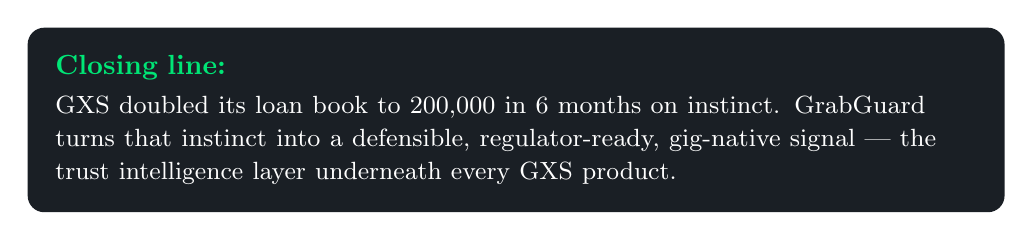
\begin{tikzpicture}
    \node[fill=GrabMid,rounded corners=6pt,text width=\linewidth-12pt,inner sep=10pt]{%
      \textcolor{GrabAccent}{\bfseries Closing line: }\\[2pt]
      \textcolor{GrabWhite}{\small GXS doubled its loan book to 200{,}000 in 6 months on instinct.
      GrabGuard turns that instinct into a defensible, regulator-ready, gig-native signal
      \textemdash{} the trust intelligence layer underneath every GXS product.}
    };
  \end{tikzpicture}
\end{frame}

% ─── SLIDE 15 — CLOSING ───
\begin{frame}[plain]
  \begin{tikzpicture}[remember picture,overlay]
    % slim GrabGreen accent band at the bottom (not full-bleed)
    \fill[GrabGreen]
      ([yshift=0.9cm]current page.south west) --
      ([yshift=1.5cm]current page.south east) --
      (current page.south east) --
      (current page.south west) -- cycle;
  \end{tikzpicture}

  \vspace*{1.8cm}
  \begin{center}
    {\fontsize{42}{46}\selectfont\bfseries\color{GrabWhite} GrabGuard}\\[0.35cm]
    {\large\color{GrabWhite} Fraud protection that treats gig income as income, not anomaly.}\\[0.25cm]
    {\footnotesize\color{GrabGray} 6 agents \textbullet\ 1 explainable model \textbullet\ 9M+ workers protected}\\[1.0cm]

    \tagpill{\faGithub\, github.com/ansh-0069/fraud\_agent}\quad
    \tagpill{\faShield\, MAS FEAT ready}\quad
    \tagpill{\faBolt\, Groq sub-200ms}\\[1.0cm]

    {\normalsize\color{GrabWhite}\bfseries
      We don't freeze accounts. We freeze fraud.}
  \end{center}
\end{frame}

\end{document}
